% $Header: /home/vedranm/bitbucket/beamer/solutions/conference-talks/conference-ornate-20min.en.tex,v 90e850259b8b 2007/01/28 20:48:30 tantau $

\documentclass{beamer}

% This file is a solution template for:

% - Talk at a conference/colloquium.
% - Talk length is about 20min.
% - Style is ornate.



% Copyright 2004 by Till Tantau <tantau@users.sourceforge.net>.
%
% In principle, this file can be redistributed and/or modified under
% the terms of the GNU Public License, version 2.
%
% However, this file is supposed to be a template to be modified
% for your own needs. For this reason, if you use this file as a
% template and not specifically distribute it as part of a another
% package/program, I grant the extra permission to freely copy and
% modify this file as you see fit and even to delete this copyright
% notice. 


\mode<presentation>
{
  \usetheme{boxes}
  \usecolortheme{seagull}
  % or ...

  \setbeamercovered{transparent}
  % or whatever (possibly just delete it)
}

\setbeamertemplate{blocks}[rounded][shadow=true]

\usepackage[czech]{babel}
% or whatever

\usepackage[utf8]{inputenc}
% or whatever

\usepackage{hyperref}
\hypersetup{colorlinks=true}

\usepackage{times}
\usepackage[T1]{fontenc}
% Or whatever. Note that the encoding and the font should match. If T1
% does not look nice, try deleting the line with the fontenc.


\title[Open Source] % (optional, use only with long paper titles)
{Open Source projekty a INSPIRE}

\subtitle {Co dělají týmy programátorů Open Source pro INSPIRE?}

\author[J. Čepický] % (optional, use only with lots of authors)
{Jáchym~Čepický\inst{1}}
% - Give the names in the same order as the appear in the paper.
% - Use the \inst{?} command only if the authors have different
%   affiliation.

\institute % (optional, but mostly needed)
{
  \inst{1}%
  Help Service - Remote Sensing s.r.o. \\
  Benešov\\
  \url{http://hsrs.cz}\\
  \
}
  
% - Use the \inst command only if there are several affiliations.
% - Keep it simple, no one is interested in your street address.

\date[27.5.2013-28.5.2013] % (optional, should be abbreviation of conference name)
{Geoinformace ve veřejné správě, 2013}
% - Either use conference name or its abbreviation.
% - Not really informative to the audience, more for people (including
%   yourself) who are reading the slides online

% If you have a file called "university-logo-filename.xxx", where xxx
% is a graphic format that can be processed by latex or pdflatex,
% resp., then you can add a logo as follows:

\pgfdeclareimage[height=1.cm]{conference-logo}{imgs/conference-logo.png}
\pgfdeclareimage[height=.5cm]{hsrs-logo}{imgs/hsrs.png}
\pgfdeclareimage[height=1.0cm]{osgeo-logo}{imgs/osgeo.png}
\pgfdeclareimage[height=.5cm]{geoserver-logo}{imgs/geoserver-logo.png}
\pgfdeclareimage[height=.5cm]{pycsw-logo}{imgs/pycsw-logo.png}
\pgfdeclareimage[height=.5cm]{geon-logo}{imgs/geon-logo.png}
\pgfdeclareimage[height=.5cm]{qgis-logo}{imgs/qgis-logo.png}
\pgfdeclareimage[height=.5cm]{ol-logo}{imgs/ol-logo.png}
\pgfdeclareimage[height=.5cm]{mapserver-logo}{imgs/mapserver-logo.png}
\pgfdeclareimage[height=.5cm]{deegree-logo}{imgs/deegree-logo.png}
\pgfdeclareimage[height=.5cm]{inspire-logo}{imgs/inspire-logo.png}
%\pgfdeclareimage[height=2.0cm]{-logo}{university-logo-filename}
\logo{\pgfuseimage{conference-logo}}



% Delete this, if you do not want the table of contents to pop up at
% the beginning of each subsection:
\AtBeginSubsection[]
{
\logo{\pgfuseimage{conference-logo}}
  \begin{frame}<beamer>{Obsah}
    \tableofcontents[currentsection,currentsubsection]
  \end{frame}
}


% If you wish to uncover everything in a step-wise fashion, uncomment
% the following command: 

%\beamerdefaultoverlayspecification{<+->}


\begin{document}

\begin{frame}
  \titlepage
\end{frame}

\begin{frame}{Obsah}
  \tableofcontents
  % You might wish to add the option [pausesections]
\end{frame}


% Structuring a talk is a difficult task and the following structure
% may not be suitable. Here are some rules that apply for this
% solution: 

% - Exactly two or three sections (other than the summary).
% - At *most* three subsections per section.
% - Talk about 30s to 2min per frame. So there should be between about
%   15 and 30 frames, all told.

% - A conference audience is likely to know very little of what you
%   are going to talk about. So *simplify*!
% - In a 20min talk, getting the main ideas across is hard
%   enough. Leave out details, even if it means being less precise than
%   you think necessary.
% - If you omit details that are vital to the proof/implementation,
%   just say so once. Everybody will be happy with that.

\section{Otevřenost, Open Source}

\begin{frame}{Open Source?}
  % - A title should summarize the slide in an understandable fashion
  %   for anyone how does not follow everything on the slide itself.

\begin{block}{Definice podle Open Source iniciativy}
    Software, jehož licence umožňuje zejména \footnote{http://opensource.org/docs/definition.html}:
    \begin{itemize} 
        \item Volné šíření
        \item Přístup ke zdrojovému kódu
        \item Vytváření odvozené práce
        \item \dots
    \end{itemize}
\end{block}
\end{frame}

\begin{frame}{Otevřenost}
    
    \begin{quote}
        Otevřenost není tisková zpráva nebo případnová studie, ale akce a dialog.
        {\em[Chris Holmes]}\footnote{http://cholmes.wordpress.com/2013/05/14/opening-esri/}
    \end{quote}

    \only<1> {
        \begin{center}
            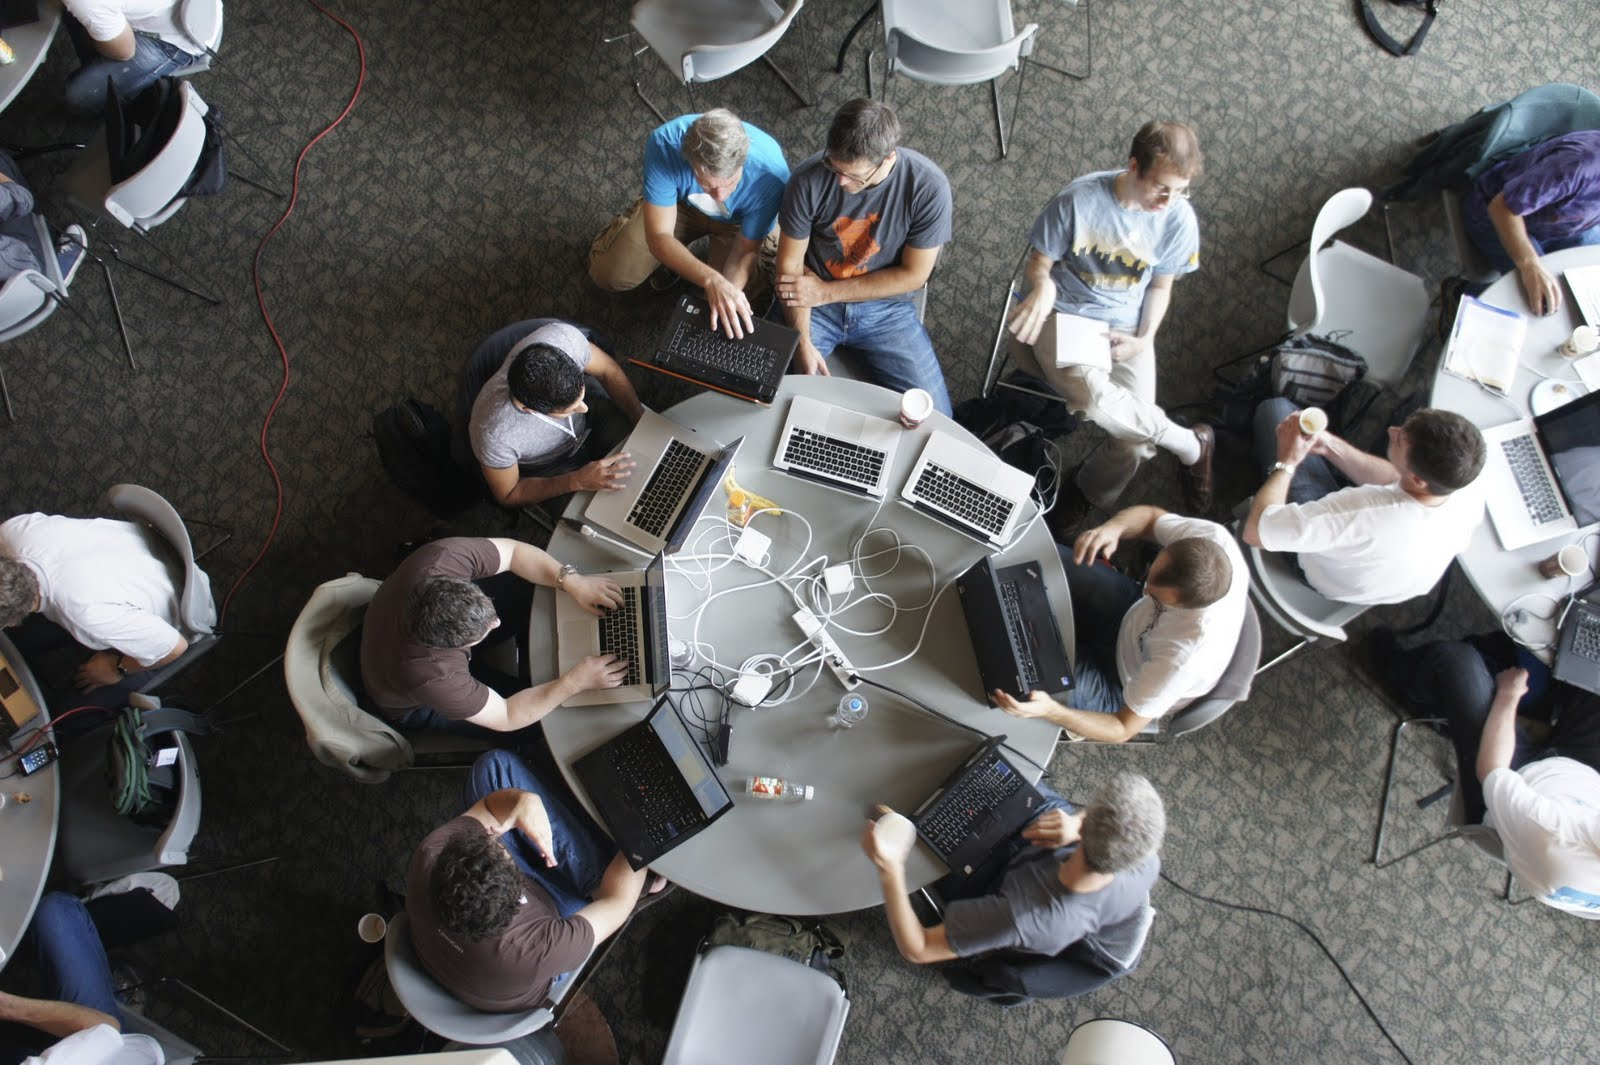
\includegraphics[width=\textheight]{imgs/ils/openess.jpg}
        \end{center}
    }
    \pause
    \only<2->{
        \begin{itemize}
            \item Upřednostnit otevřené služby a formáty proprietárními
                \pause
            \item Poskytnout dokumentaci k propritárním službám a formátům
                \pause
            \item Diskuse na otevřených fórech, naslouchání opozičních názorů
            \item \dots
        \end{itemize}
    }% /only
\end{frame}

\begin{frame}{Otevřenost = svoboda pohybu}
        \begin{center}
            
\includegraphics[width=\textheight]{imgs/ils/open-door.jpg}
        \end{center}
        
\end{frame}

\begin{frame}{Otevřenost $=$ spolupráce}
        \begin{center}
            
\includegraphics[width=\textheight]{imgs/ils/escher.jpg}
        \end{center}
\end{frame}

\begin{frame}{Otevřenost $=$ spolupráce}
    \begin{itemize}
        \item Programování (GNU/Linux, GRASS GIS, MapServer, Firefox, Chromium,
        Android, \dots)
            \pause
        \item Informace (Wikipedia)
            \pause
        \item Data (Open Data, OpenStreetMap, OpenAerialMap, GrassRootsMapping,
        \dots)
    \end{itemize}
\end{frame}

\logo{\pgfuseimage{osgeo-logo}}
\section{Open Source Geospatial foundation}

\begin{frame}{OSGeo}
\begin{block}{Open Source Geospatial Foundation -- \href{http://osgeo.org}{OSGeo}}
Nezisková organizace, jejíž cíl je podpora společného vývoje otevřeného software
pro geinformatiku a podpora jeho užívání. 

Poskytuje finanční, organizační a právní podporu široké geoprostorové komunitě.
Slouží jako nezávislá právnická osoba, na kterou mohou její členové převézt
výsleky své práce (přispívat do zdrojového kódu, přispět finanční částkou a
dalšími zdroji) pro obecné blaho. {\em Certifikace projektů}

OSGeo požívá status US 501(c)(3) neziskové organizace.
\end{block}
\end{frame}

\begin{frame}{OSGeo Struktura}
    Představenstvo OSGeo
    \begin{center}
    \only<1>{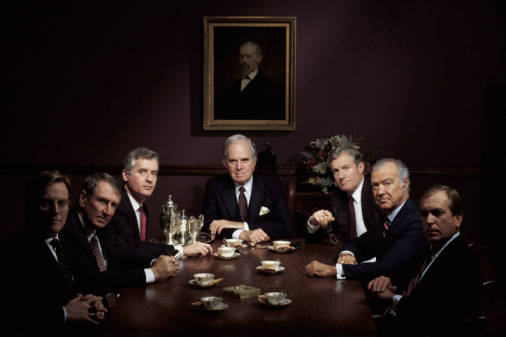
\includegraphics[height=3.5cm]{imgs/ils/board.jpg}}
    \only<2>{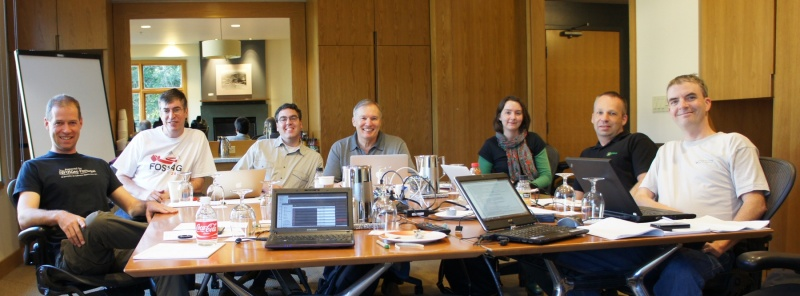
\includegraphics[height=3.5cm]{imgs/ils/osgeo-board.jpg}}
    \only<3->{
\includegraphics[height=3.5cm]{imgs/ils/osgeo-irc.png}}
    \end{center}

    \uncover<4>{
        \begin{itemize}
            \item Peter Batty, Jáchym Čepický, Michael Gerlek, Anne Ghisla, Mark Lucas,
            {\bf Jeff McKenna}, Daniel Morissette, Cameron Shorter, Frank Warmerdam
        \end{itemize}
}
\end{frame}
\begin{frame}{OSGeo Struktura}
\begin{itemize}
    \item Peter Batty, Jáchym Čepický, Michael Gerlek, Anne Ghisla, Mark Lucas,
        {\bf Jeff McKenna}, Daniel Morissette, Cameron Shorter, Frank Warmerdam
    \item Základní členové (s volčiským právem, 144)
            \pause
    \item Lokální skupiny  (20+)
            \pause
    \item Pracovní skupiny (Website, Finance, Incubation, {\em Education, Conference})
\end{itemize}
\end{frame}

\logo{\pgfuseimage{inspire-logo}}
\section{INSPIRE v OSGeo}

\begin{frame}{INSPIRE v OSGeo}
    \begin{itemize}
        \item Nově se formuje
            \href{http://wiki.osgeo.org/wiki/SDI_committee}{pracovní skupina pro
            SDI} (se zaměřením na INSPIRE)
        \item Analýza současného stavu provedena na
            \url{http://wiki.osgeo.org/wiki/INSPIRE} {\em } 
    \end{itemize}
\end{frame}

\subsection{Prohlížecí služby}
\logo{\pgfuseimage{osgeo-logo}}
\begin{frame}{Prohlížecí služby -- Server}
    \begin{itemize}
        \item \href{http://mapserver.org}{MapServer}
        \item \href{http://geoserver.org}{GeoServer}
        \item \href{http://deegree.org}{deegree}
        \item \href{http://mapguide.osgeo.org}{MapGuide}
    \end{itemize}
    \begin{flushright} 
\includegraphics[width=2cm]{imgs/ils/done.jpg} \end{flushright} 
\end{frame}

\begin{frame}{Prohlížecí služby -- Client}
    \begin{itemize}
        \item \href{http://openlayers.org}{OpenLayers}
        \item \href{http://qgis.org}{QGIS}
    \end{itemize}
    \begin{flushright} 
\includegraphics[width=2cm]{imgs/ils/done.jpg} \end{flushright}
\end{frame}

\subsection{Vyhledávací služby}
\logo{\pgfuseimage{osgeo-logo}}
\begin{frame}{Vyhledávací služby}
    \begin{itemize}
        \item \href{http://geonetwork-opensource.org}{GeoNetwork}
        \item \href{http://deegree.org}{deegree}
        \item \href{http://pycsw.org}{pycsw}
    \end{itemize}
    \begin{flushright} 
\includegraphics[width=2cm]{imgs/ils/done.jpg} \end{flushright}
\end{frame}

\subsection{Stahovací služby}
\logo{\pgfuseimage{osgeo-logo}}
\begin{frame}{Stahovací služby}
    \begin{itemize}
        \item \href{http://geoserver.org}{GeoServer}
        \item \href{http://mapserver.org}{MapServer}
        \item \href{http://deegree.org}{deegree}
    \end{itemize}
    \begin{flushright}
\includegraphics[width=2cm]{imgs/ils/done.jpg}\end{flushright}
\end{frame}


\subsection{Jak pokračují práce}
\begin{frame}{Pokračující práce}
    \begin{center} 
        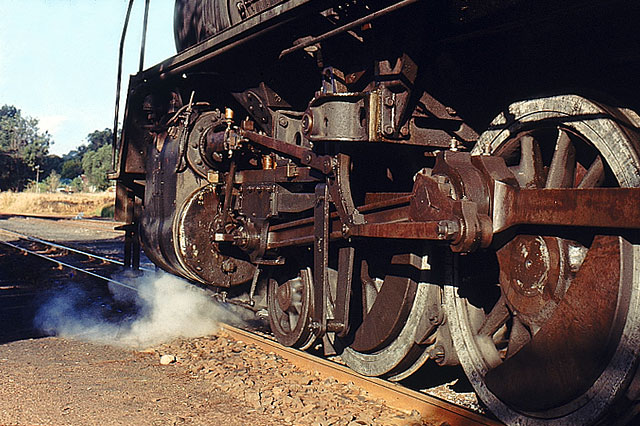
\includegraphics[width=\textwidth]{imgs/ils/engine.jpg}
    \end{center}
\end{frame}

\logo{\pgfuseimage{mapserver-logo}}

\begin{frame}{MapServer}
Vztah MapServeru k INSPIRE popisuje nelépe stránka
\url{http://mapserver.org/ogc/inspire.html}. 

\begin{itemize}
    \item 6.0.3 (květen 2012)
        \begin{itemize}
            \item Pořadí os v souřadnicích u WCS
            \item Oprava rozlišení pro různé jednotky u WCS
            \item Oprava WCS GetCapabilities, přidání metadat
        \end{itemize}
        \pause
    \item 6.2.0 (listopad 2012)
        \begin{itemize}
            \item Kompletní podpora INSPIRE View Service
        \end{itemize}
        \pause
    \item 6.2.1 (duben 2013)
        \begin{itemize}
            \item Opravy v GetCapabilities dokumentu
        \end{itemize}
\end{itemize}
\end{frame}

\logo{\pgfuseimage{geoserver-logo}}
\begin{frame}{GeoServer}
    GeoSolutions: Analýza GeoServeru z pohledu
    INSPIRE\footnote{{Analysing GeoServer compatibility with INSPIRE requirements}}.
Od verze 2.1.0 lze doinstalovat speciální rozšíření INPSIRE, upravující View
Service metadata a další.
    \begin{itemize}
        \item 2.1.4 (červen 2012)
            \pause
        \item 2.2.2 (říjen 2012) Oprava INSPIRE rozšíření a GetFetureInfo
            \pause
        \item 2.2.5 (únor 2013) Oprava WMS GetLegendGraphic, oprava velikosti
        pixelu u WCS
            \pause
        \item 2.3.0 (březen 2013) Opravy WCS 2.0.0, \dots
            \pause
        \item 2.3.2 (květen 2013) Komunitní INSPIRE modul se stal oficiálním
            rozšířením
    \end{itemize}
\end{frame}

%\begin{frame}{GeoServer}
%\begin{itemize}
%    \item View Services
%    \begin{itemize}
%        \item Podpora pro WMS 1.3, upravená metadata GetCapabilies, 
%        \item Podpora pro multi-jazyčné popisy
%        \item Podpora požadovaných souř. systémů a formátů
%        \item Podpora pro SLD
%    \end{itemize}
%    \pause
%    \item Download service
%    \begin{itemize}
%        \item GML 3.2.1
%        \item \dots
%    \end{itemize}
%\end{itemize}
%\end{frame}

\logo{\pgfuseimage{deegree-logo}}
\begin{frame}{deegree}
\href{http://deegree.org}{Deegree} je vyvíjen v Německu a okamžitě nasazován u měst (Bonn) a ve státní
správě. Deegree byl vybrán pro INSPIRE geoportál.

Více informací o deegree a INSPIRE na
\url{http://wiki.deegree.org/deegreeWiki/InspireNode}

3.2.0-3.2.3 (březen - duben 2013) - Opravy INSPIRE download service a View service
\end{frame}

\logo{\pgfuseimage{geon-logo}}
\begin{frame}{GeoNetwork}
Mezi verzemi 2.6 a 2.8 jsou dva roky práce.
    \begin{itemize}
        \item Přidání vlastní parametrů do CSW
        \item Verzování metadatového záznamu
        \item Rozhranní pro GeoServer (přímé nahrávání dat)
        \item \dots (více než 500 změn)
    \end{itemize}
\end{frame}

\logo{\pgfuseimage{pycsw-logo}}
\begin{frame}{PyCSW}
    \href{http://pycsw.org}{PyCSW} je nový projekt (2011), zatím není součástí OSGeo. 
    \begin{itemize}
        \item Katalogový server/klient
        \item Bez grafického rozhraní
        % \item Referenční implementace OSGeo
    \end{itemize}
\end{frame}

\logo{\pgfuseimage{qgis-logo}}
\begin{frame}{QGIS}
    Desktopová prohlížečka dat, obsahuje WMS, WFS klienty, možnost editace dat.
    Zásuvné moduly pro INSPIRE:
    \begin{itemize}
        \item Atom klient (INSPIRE Download service 3.0)
        \item WFS 2.0 klient
        \item qgCSW - CSW metadatový klient
        \item \dots
    \end{itemize}
\end{frame}

\logo{\pgfuseimage{ol-logo}}
\begin{frame}{OpenLayers}
    \href{http://openlayers.org}{OpenLayers} Webový mapový framework, používaný
    často jako základ pro nadstavby (\href{http://hslayers.org}{HSLayers},
    \href{http://geoext.org}{GeoExt}, InterGraph Geoportál, \dots)

    \begin{itemize}
        \item Použitelný jako klient prohlížecí, stahovací (i transformační) služby
        \item Ovládání zcela podle požadavků INSPIRE
    \end{itemize}

    Často je jim vytýkána velikost. Žádný další JavaScriptový framework není ale
    tak komplexní.
\end{frame}

\logo{\pgfuseimage{conference-logo}}
\section{Open source aktivity v ČR}
\begin{frame}{OS v ČR}
    \begin{itemize}
        \item \href{http://www.cagi.cz/os25-open-source-a-open-data}{Odborná skupina CAGI} \\
            Jáchym Čepický (Help Service - Remote Sensing), Aleš Čepek (FSV, ČVUT),\\
            Otakar Čerba (FAV, ZČU), Přemysl Vohnout (CCSS),\\
            Rostislav Nétek (PřF, ÚPOL), Ladislav Čapek (Geosense)
        \pause

        \item Občanské sdružení OSGeo-czech \href{mailto:freegeocz@fsv.cvut.cz}{freegeocz@fsv.cvut.cz}
            \pause
        \item Konference Geoinformatics \url{http://geoinformatics.fsv.cvut.cz/}
            11-12 červenec 2013, GRASS GIS Community Sprint in Prague, Czech
            Republic 12-18 červenec, 2013
            \pause
        \item OpenStreetMap conference \href{mailto:talk-cz@openstreetmap.org}{talk-cz@openstreetmap.org}
    \end{itemize}
\end{frame}



\logo{\pgfuseimage{hsrs-logo}}
\section*{Závěr}

\begin{frame}{Závěr}

  % Keep the summary *very short*.
  \begin{itemize}
  \item
    Projekty OSGeo intenzivně pracují na jejich používání v rámci SDI
  \item
    Z pohledu OSGeo je INSPIRE jednou z klíčových iniciativ, všechny projekty se
    snaží o úpravy směrem k INSPIRE
  \item Open Source není jediná správná cesta. Je to jiná správná cesta --
      Open Source může být i {\em profesionální} i {\em komerční}, vždy ale
      \alert{otevřený}.

\begin{center} 
    
\includegraphics[height=4.5cm]{imgs/ils/oneway.png}
\end{center}
  
\end{itemize}
  
\end{frame}


\begin{frame}
    \begin{center}
        Jáchym Čepický \\
        jachym@hsrs.cz \\
        \url{http://bnhelp.cz/} \\
        \url{http://osgeo.org}
    \end{center}
\end{frame}

\end{document}


